%Copyright (C) 2014 Sergio García Villalonga.

A la hora de realitzar les proves de localització, és necessari uns resultats que es puguin reflectir en un conjunt de dades numèriques que reflecteixin, en el nostre cas, l'error de localització en cada posició. En el cas d'utilitzar l'AirPlace Tracker en mode "on-line", encara que el resultat és més visual, l'anàlisi depèn en gran mesura de la posició ocupada en cada moment, pel que el temps és una variable addicional que converteix la tasta en quelcom més complex.

Per altra banda, l'anàlisi "off-line", al partir d'unes dades persistents, en forma de mapa de ràdio, permet realitzar diversos estudis sobre exactament el mateix conjunt de dades, podent utilitzar diferents algorismes amb diferents paràmetres. Aquest fet és clau pel nostre estudi, ja que ens permet dur a terme un anàlisi amb més profunditat i verificar com la presència d'usuaris afecta als resultats segons variem l'algorisme i els paràmetres. També ens permet verificar quina combinació afavoreix un millor resultat en els diferents contextos.

A continuació s'exposen els detalls de la presa de dades i els resultats obtinguts del seu anàlisi.

\subsection{Presa de dades}

La presa de dades per realitzar un anàlisi "off-line" de localitzacions en interior amb l'AirPlace Tracker comença amb la creació d'un mapa de ràdio a noves localitzacions utilitzatn l'AirPlace Logger. En el nostre cas, però, se n'han hagut de crear dos mapes, a exactament la mateixes localitzacions però en diferents instants, per tal de que les mesures es veiessin afectades per la quantitat de persones presents a l'entorn. La recollida de dades amb una presència mínima de gent a l'entorn (figura \ref{fig:foto_buit}) es va dur a terme en un context similar a la de la creació del mapa de ràdio: a partir de les 8 del matí pels passadissos i a partir de les 10 dins les tendes. El segon mapa a analitzar es va intentar realitzar en un moment en que la presència de clients al centre comercial fos massiva. En concret, les dades es varen recol·lectar els dies 20 i 21 de desembre de 2014, el cap de setmana previ a les festes de Nadal. Com s'aprecia a la figura \ref{fig:foto_ple} la ocupació del centre és notable.

\begin{figure}[ht]
\begin{center}
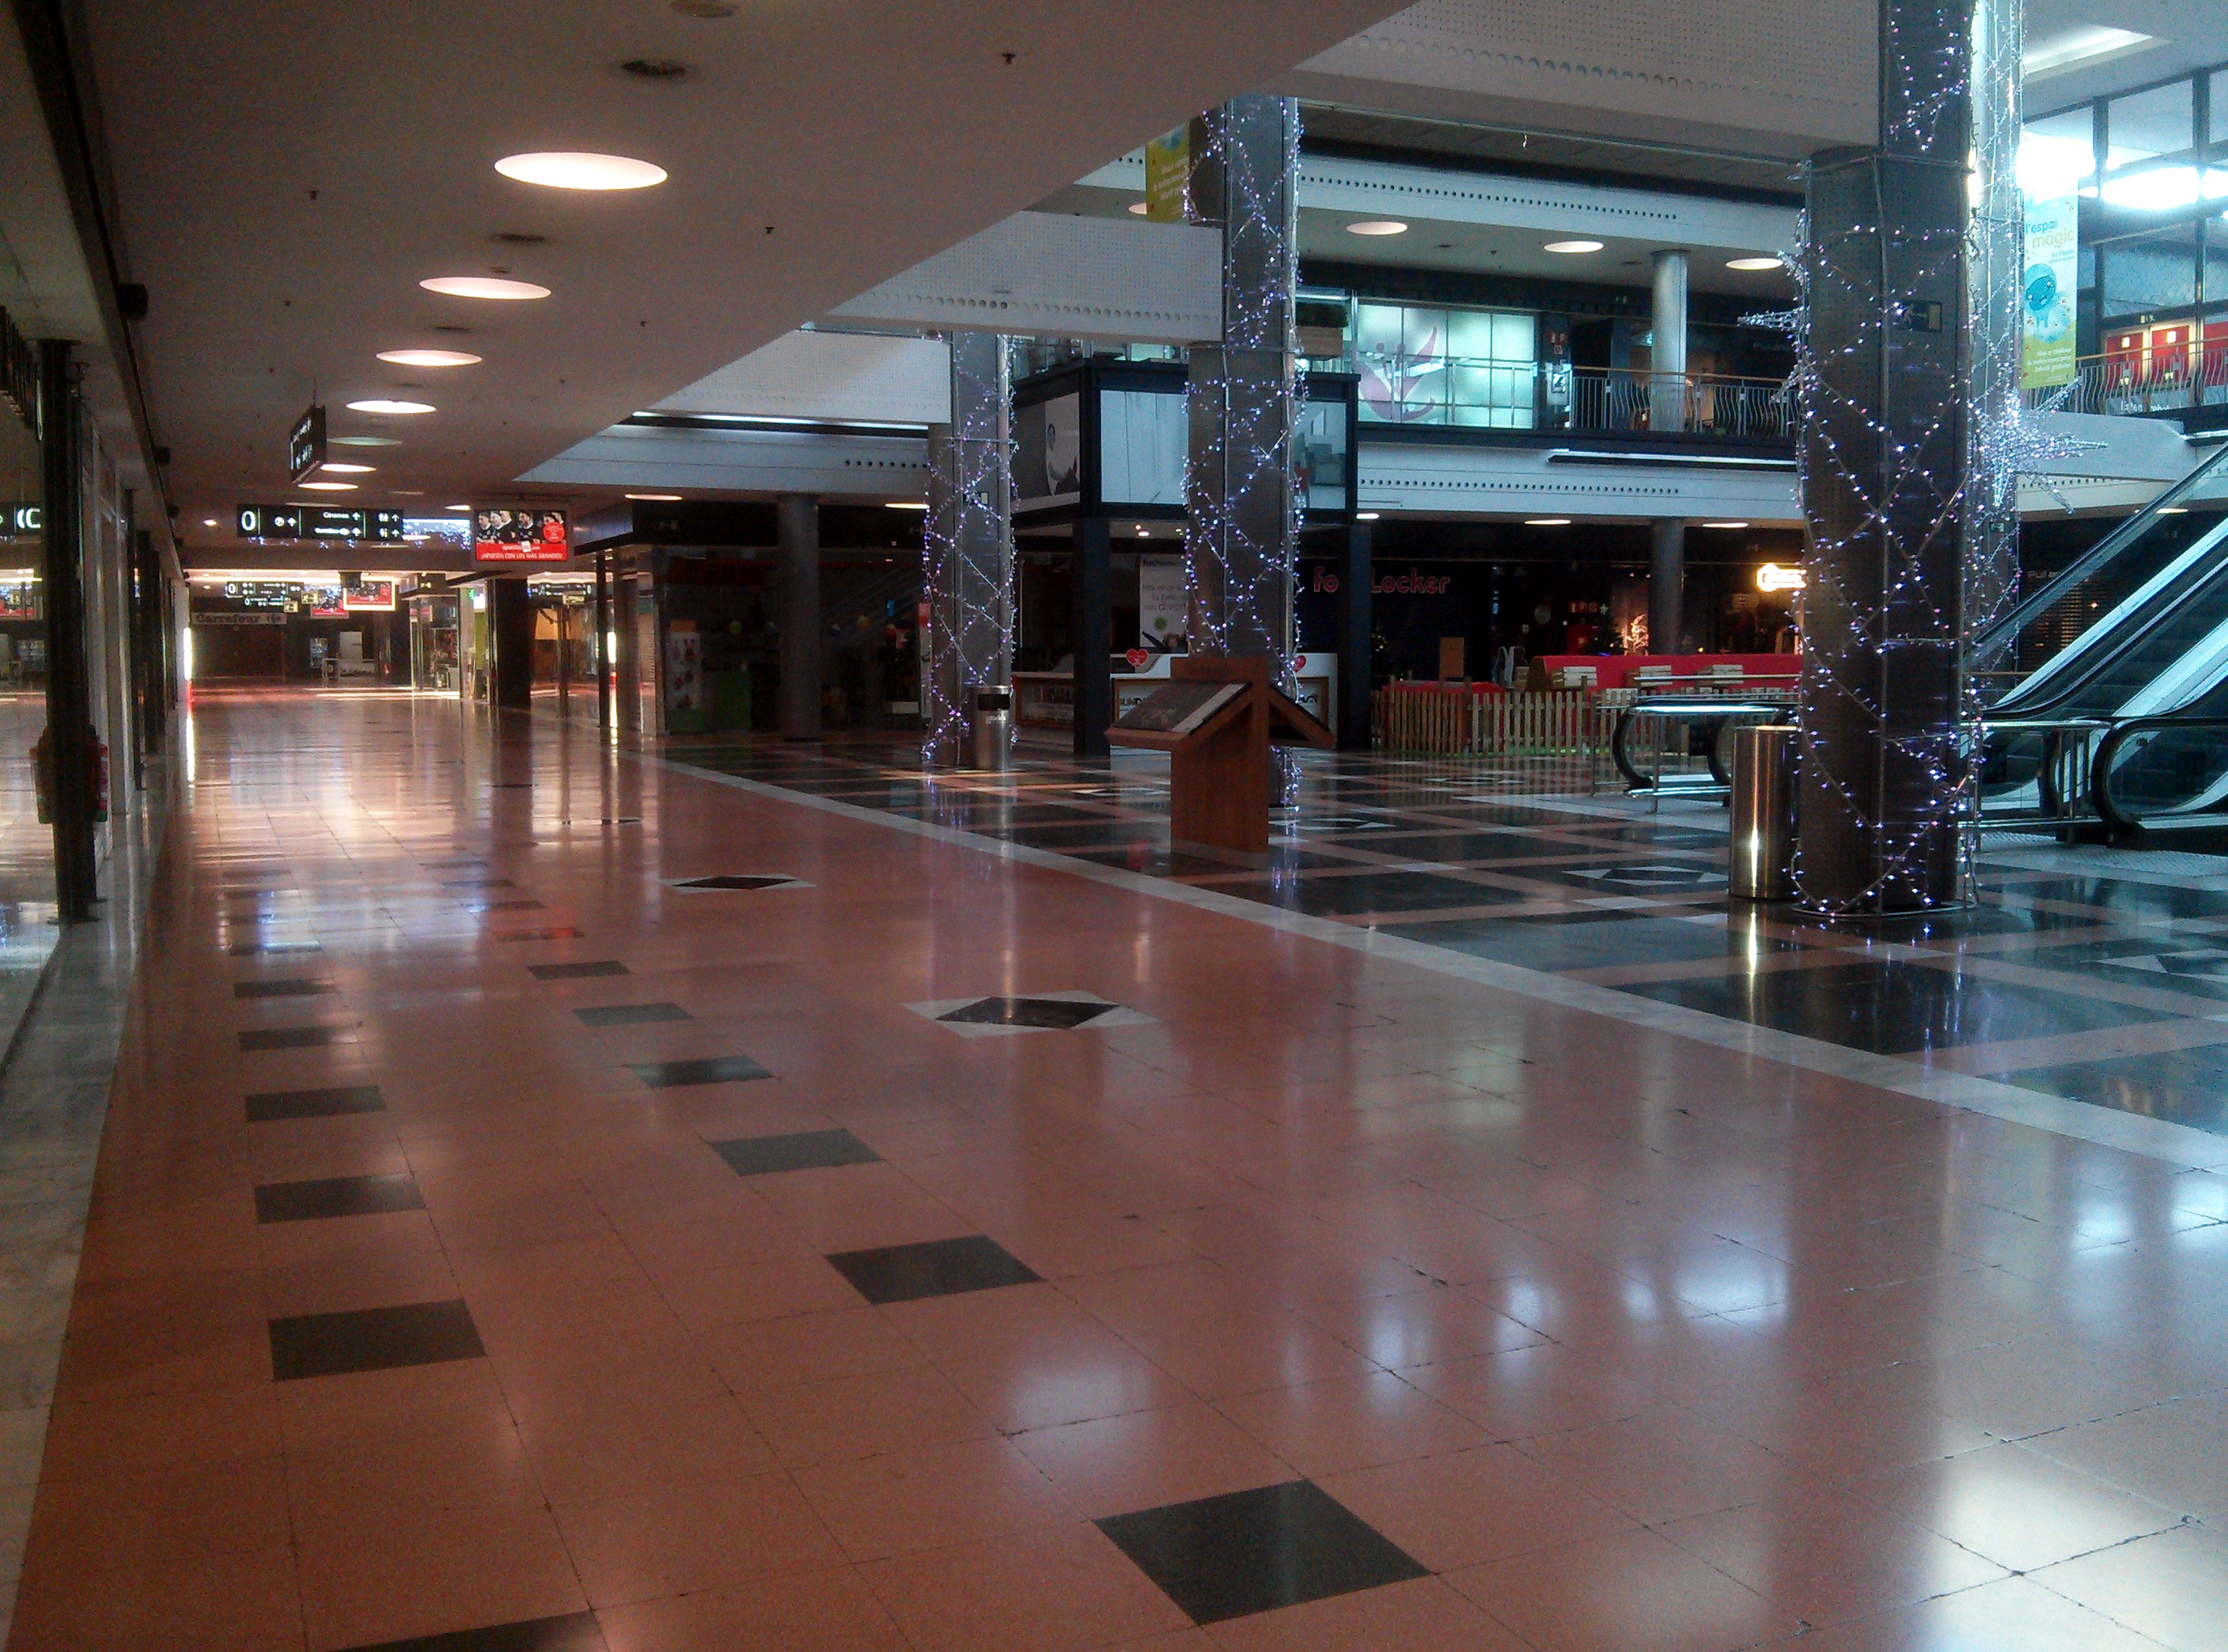
\includegraphics[width=7cm]{imatges/foto_buit.jpg}
\caption{Centre comercial en les proves sense usuaris.}
\label{fig:foto_buit}
\end{center}
\end{figure}

\begin{figure}[ht]
\begin{center}
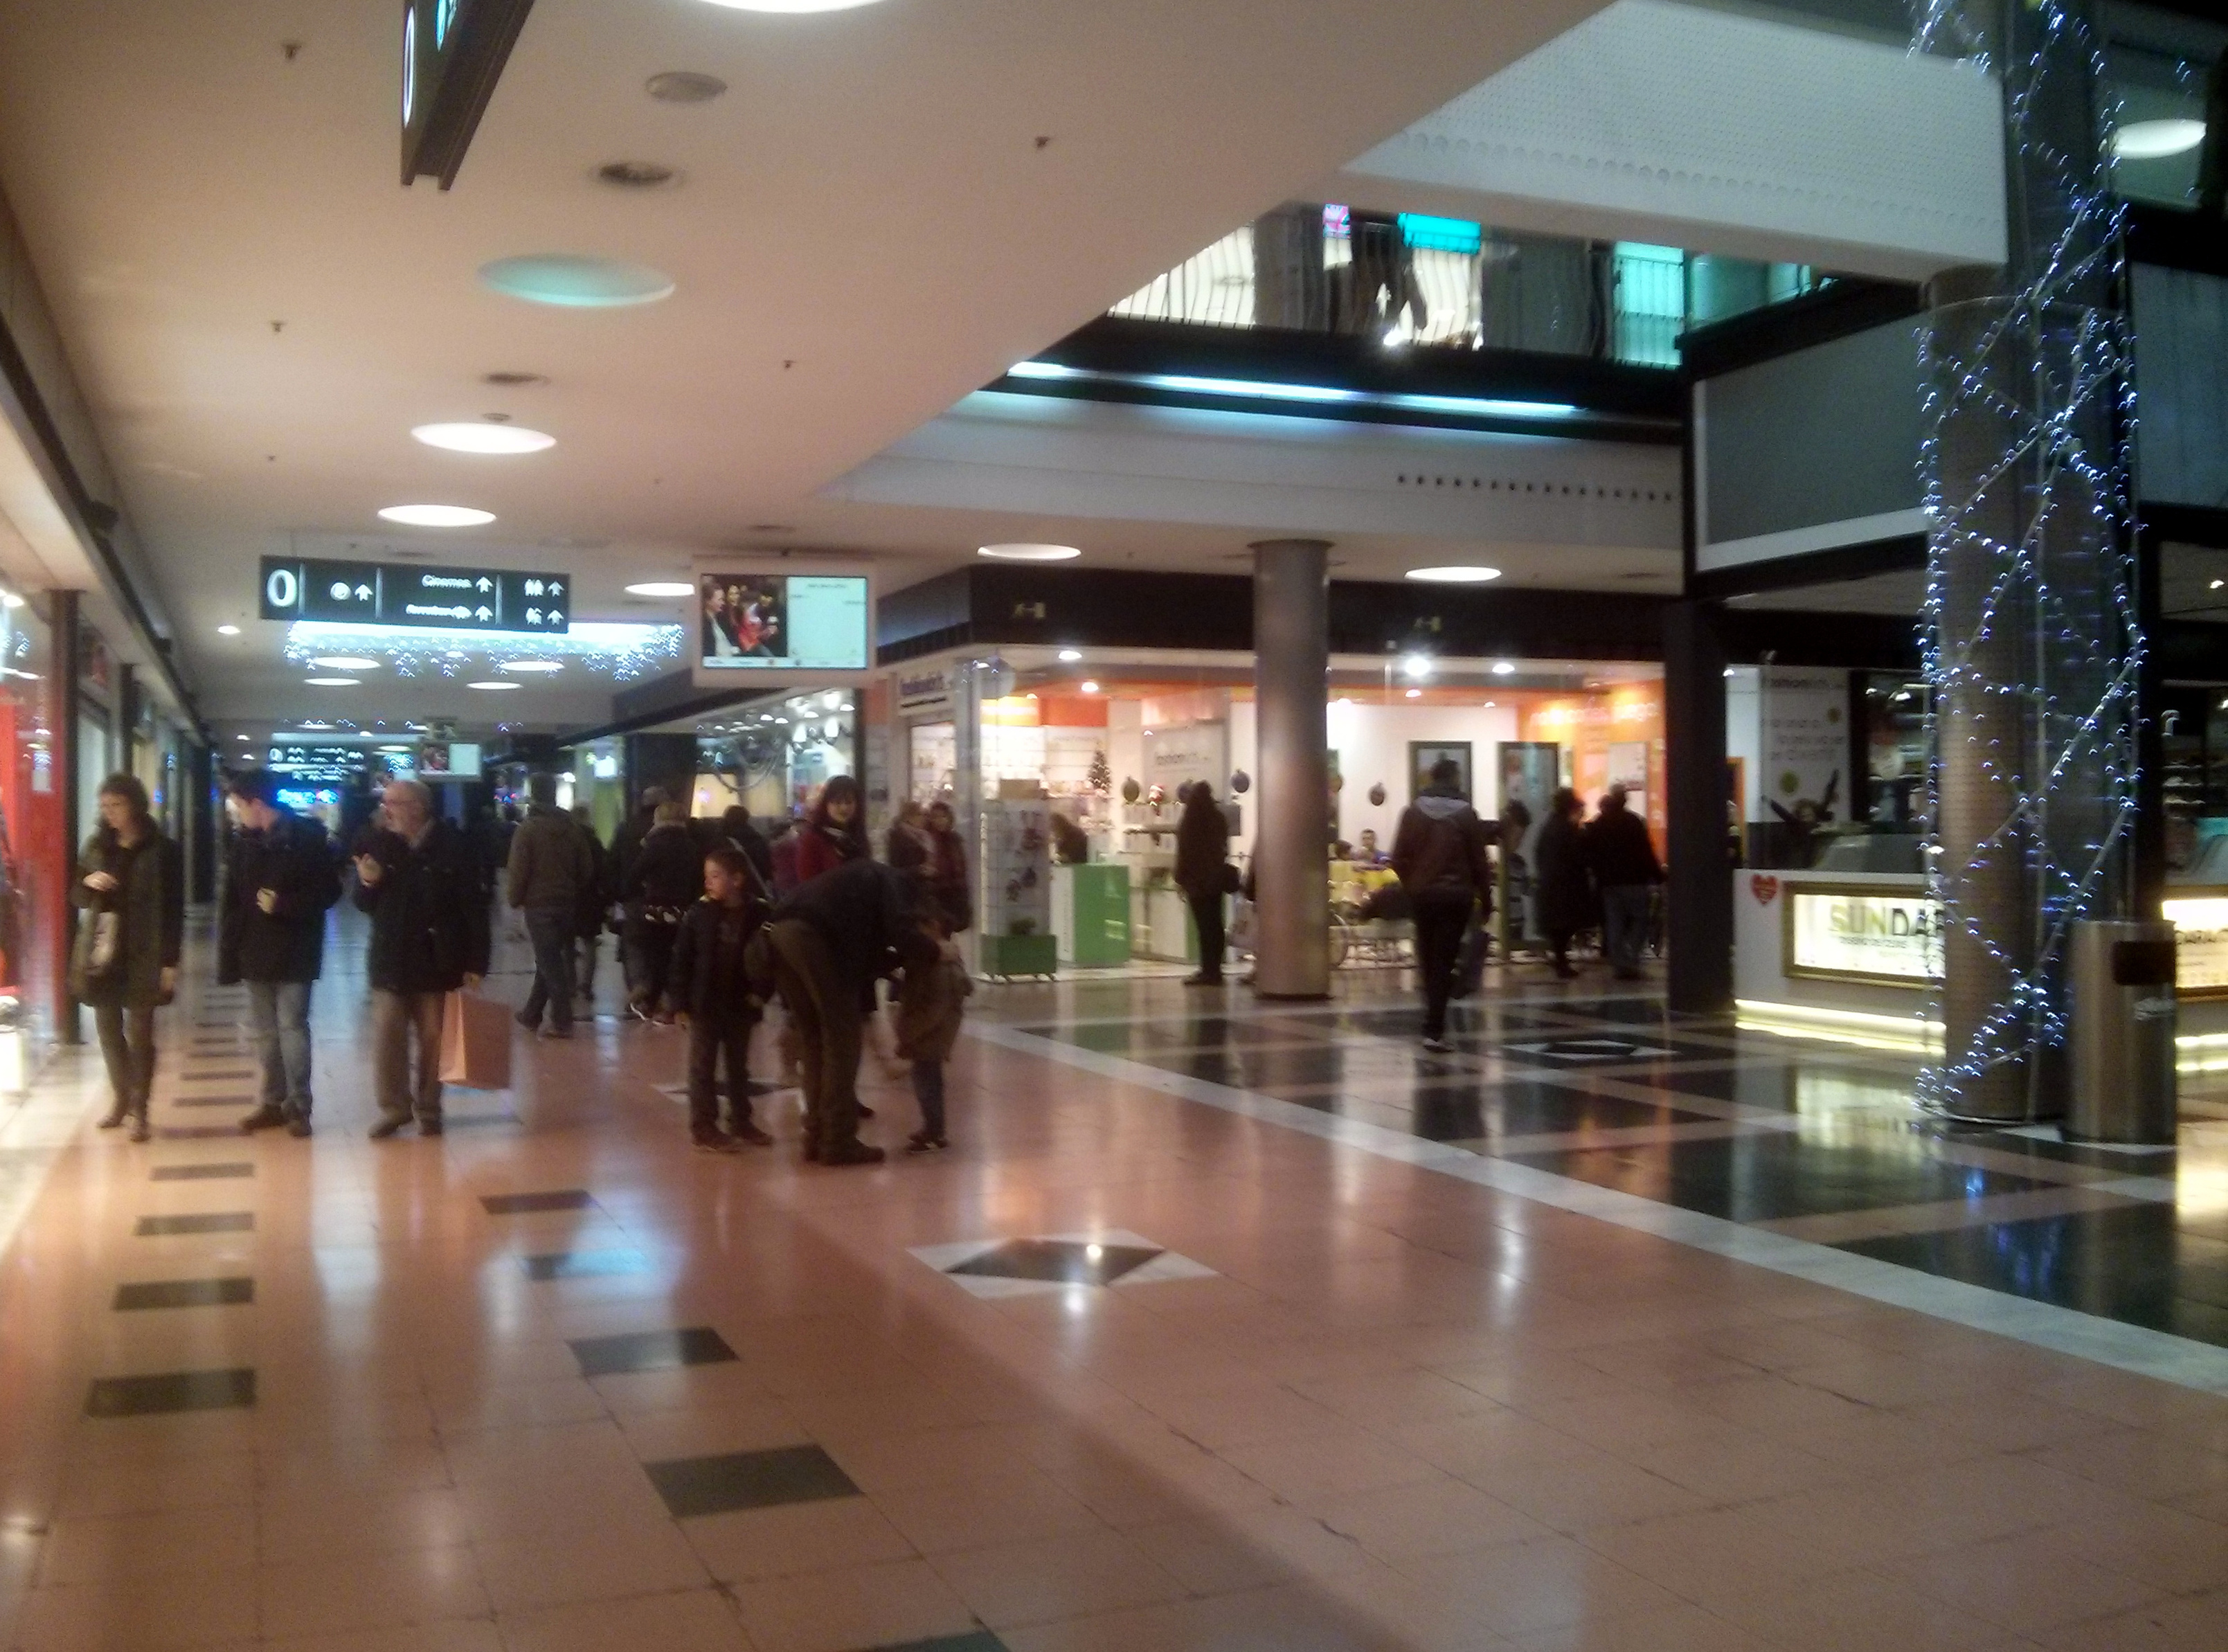
\includegraphics[width=7cm]{imatges/foto_ple.jpg}
\caption{Centre comercial en les proves en horari comercial.}
\label{fig:foto_ple}
\end{center}
\end{figure}

Com s'ha comentat, i per tal de que els resultats fossin comparatius, en ambdós contexts, les localitzacions on s'han pres les dades han estat les mateixes. Es tracta de 115 mostres a posicions diferents (figura \ref{fig:planol_proves}), de les quals 42 es troben dins tendes i 73 pels passadissos. La distància mínima mitjana entre mostres és de 5,56 m. i la distància mínima màxima en el conjunt és de 11 m.

\begin{figure}[ht]
\begin{center}
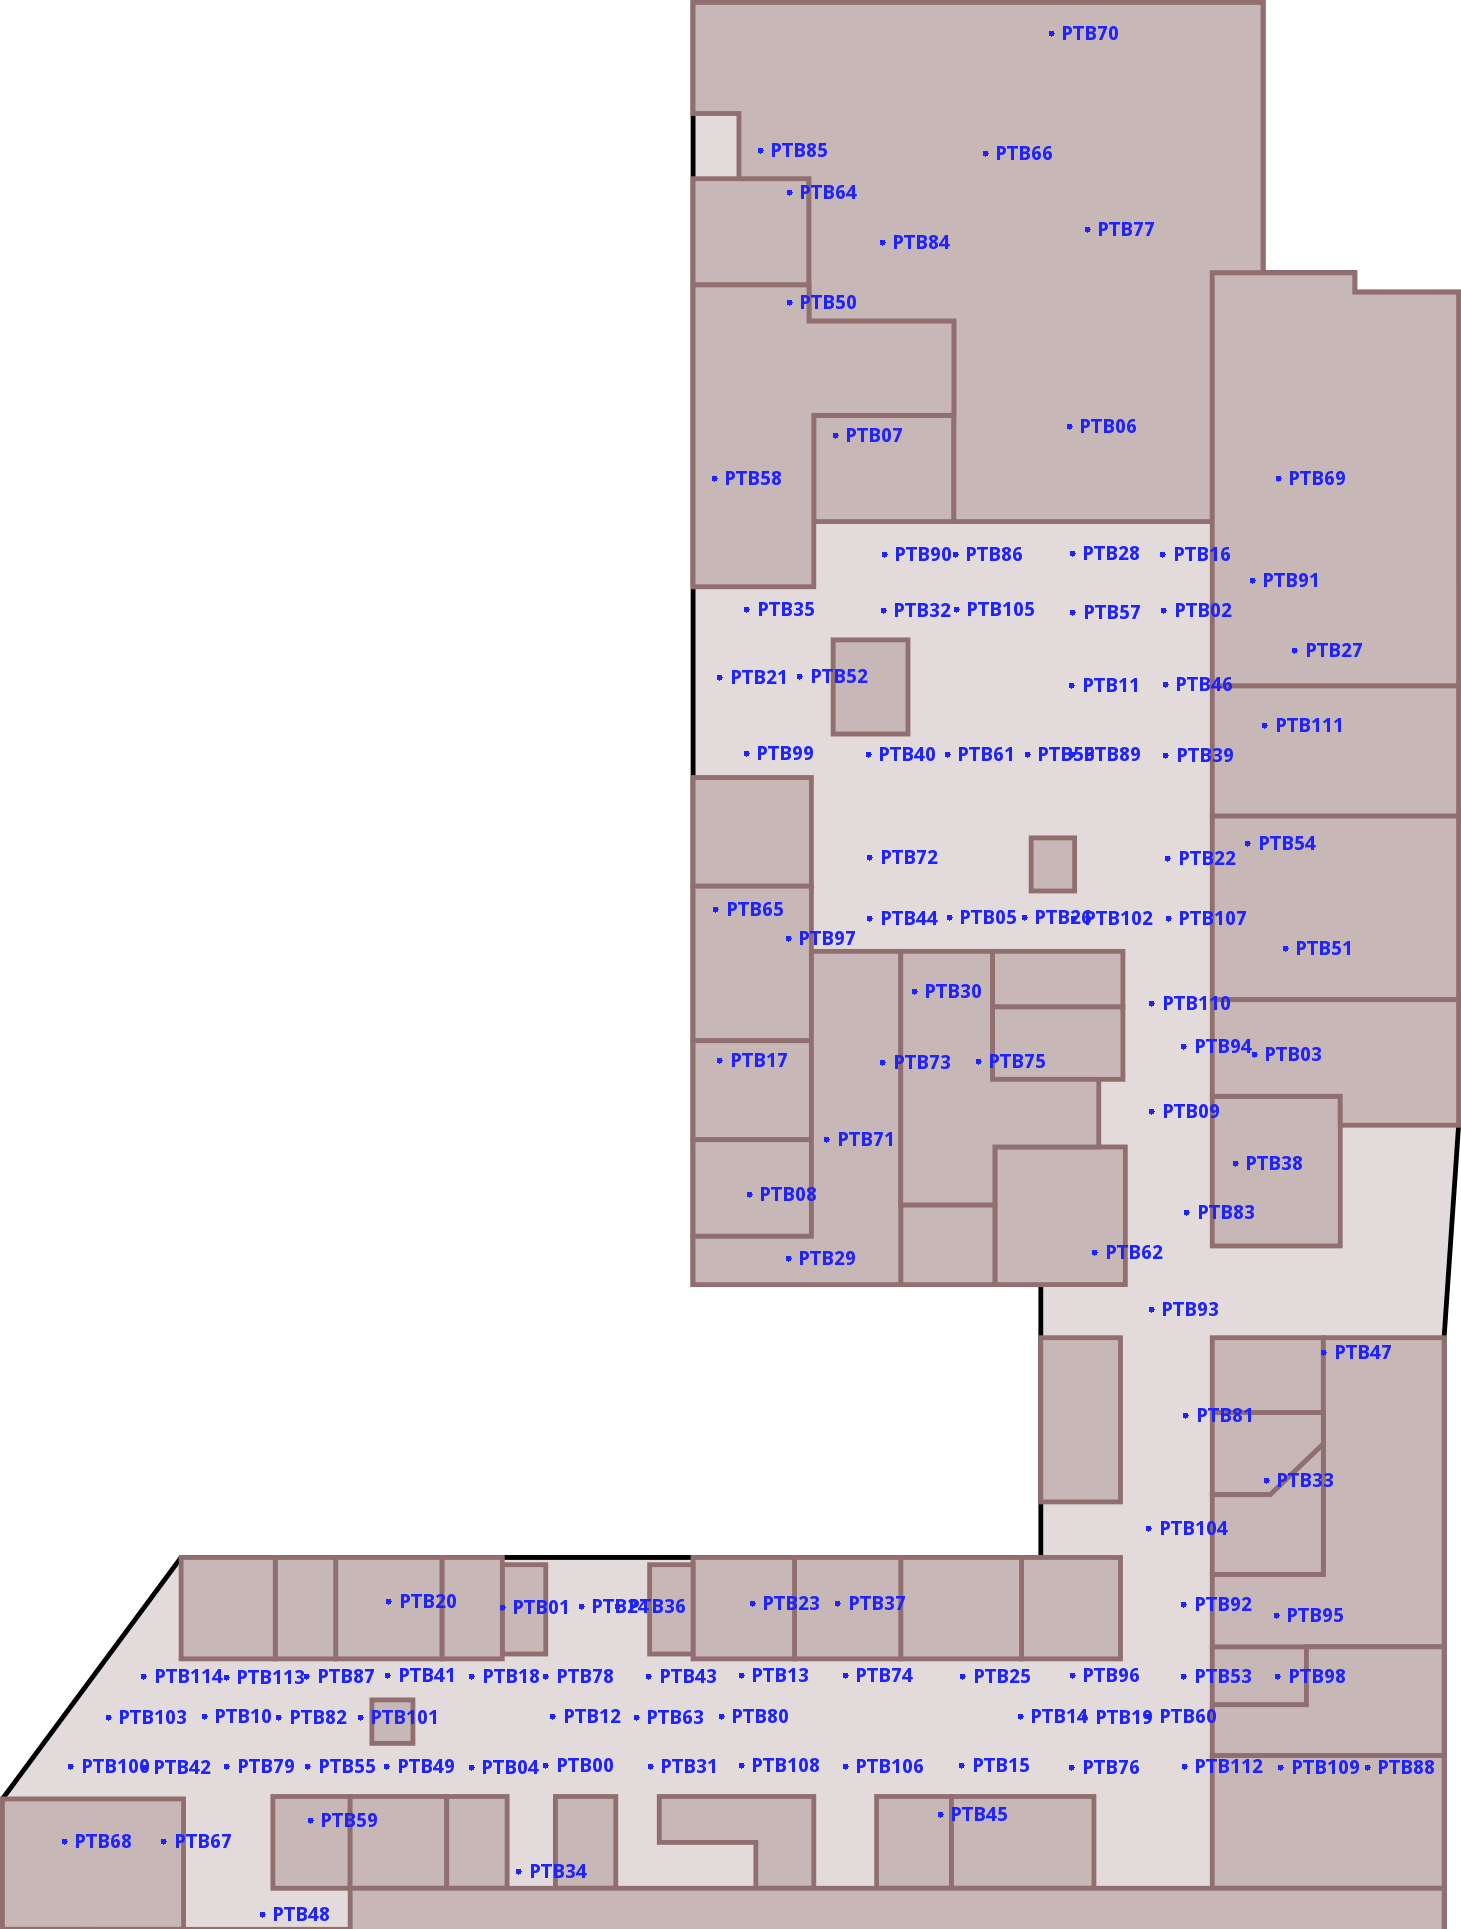
\includegraphics[width=7cm]{imatges/planol_proves.png}
\caption{Punts on s'ha dut a terme la presa de dades en les proves.}
\label{fig:planol_proves}
\end{center}
\end{figure}

\subsection{Estimació de les localitzacions de prova}

Per tal de realitzar un anàlisi detallat de les dades generades a posteriori, l'AirPlace Tracker proporciona el mode "off-line", amb el qual, donat dos mapes de radio, l'utilitzat per realitzar les estimacions en sí i un de localitzacions de prova, estima les posicions del segon i calcula l'error mitjà en les localitzacions. Aquesta operació es pot realitzar repetidament i amb diferents algorismes, pel que ens permet estudiar de manera més detallada la influència d'usuaris a l'entorn. De totes formes, el funcionament del mode "off-line" no aporta cap dada persistent per ser analitzada a posteriori, sino que després de l'anàlisi es limita a mostrar un diàleg amb estadístiques d'aquest (figura \ref{fig:analisi_offline_defecte}). Aquest tipus de resultat només ens permet saber la mitjana de l'error, però no permet, per exemple, saber la desviació mitjana de l'error o classificar els resultats de l'anàlisi en resultats en tendes i en passadissos.

\begin{figure}[ht]
\begin{center}
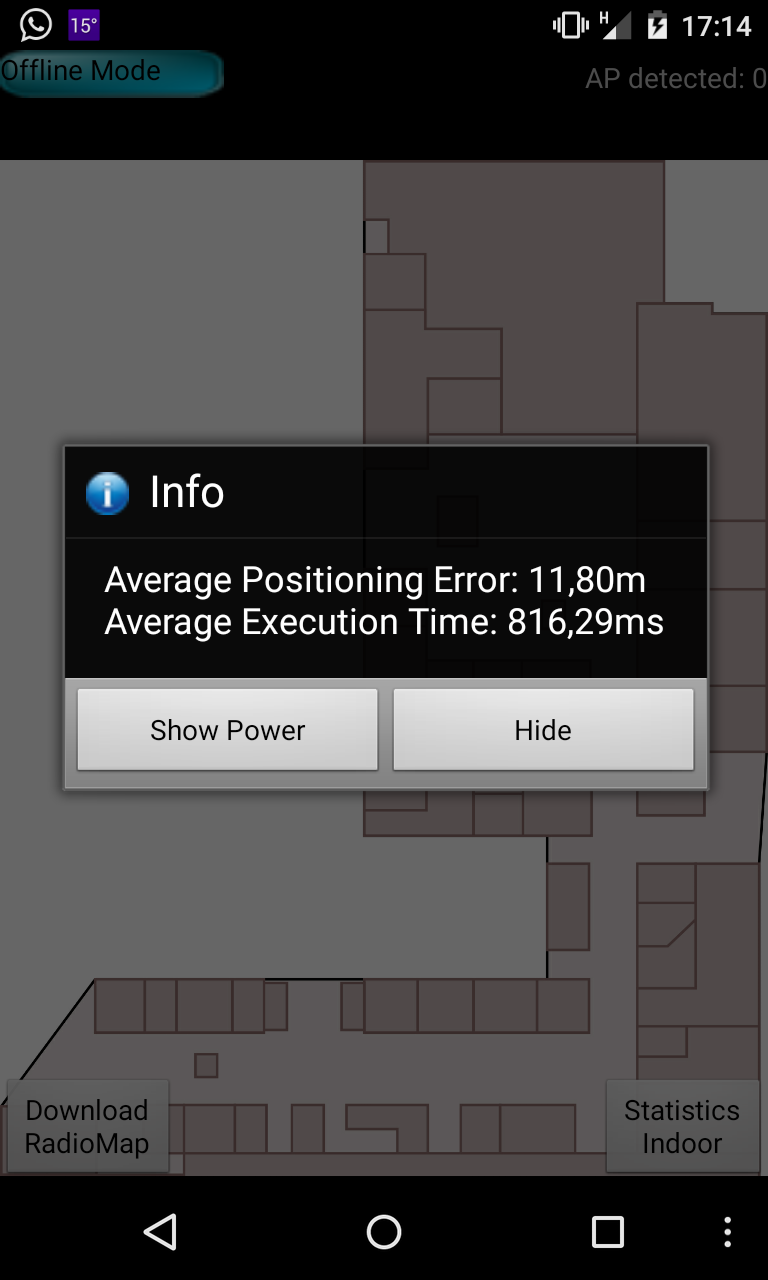
\includegraphics[width=5cm]{imatges/analisi_offline_defecte.png}
\caption{Final de l'execució d'un anàlisi off-line d'AirTracker.}
\label{fig:analisi_offline_defecte}
\end{center}
\end{figure}

Un altre problema és el temps d'execució de les proves. Malgrat que depenent de l'algorisme triat i dels paràmetres corresponents, l'anàlisi de l'error de posicions per una quantitat de localitzacions relativament gran porta, aproximadament, una mitja de 80 minuts. Aquest factor dificulta la realització d'anàlisis per diferents algorismes i paràmetres.

Aprofitant la seva llicència lliure, es va decidir realitzar una sèrie de modificacions a l'AirPlace Tracker per tal d'aprofitar millor els recursos de maquinari i poder realitzar un anàlisi més detallat \footnote{El codi modificat es pot trobar a \url{https://github.com/SeGarVi/TFM/tree/master/AirplaceTracker}}. Per tal de poder obternir resultats ilustratius, es va decidir persistir els resultats dels anàlisis. D'aquesta manera, per cada execució amb un algoritme i paràmetres concrets es genera un fitxer de text amb la posició real de cada localització, la posició estimada, i l'error.

Per altra banda, per tal de millorar els temps d'anàlisi, s'ha optat per aprofitar les característiques multinucli del processador del Nexus 4. Amb l'actual versió modificada, s'executen quatre anàlisis en paral·lel, un amb cada algoritme (figura \ref{fig:analisi_offline_paralel}). Amb aquesta modificació es logra una millora considerable, passant dels temps anteriorment mencionats, per cada algorisme, a uns 110 de mitjana aproximadament, pels quatre algorismes simultàniament, el que ens permet realitzar l'anàlisi amb diferents combinacions d'algorismes i paràmetres en un temps raonable.

\begin{figure}[ht]
\begin{center}
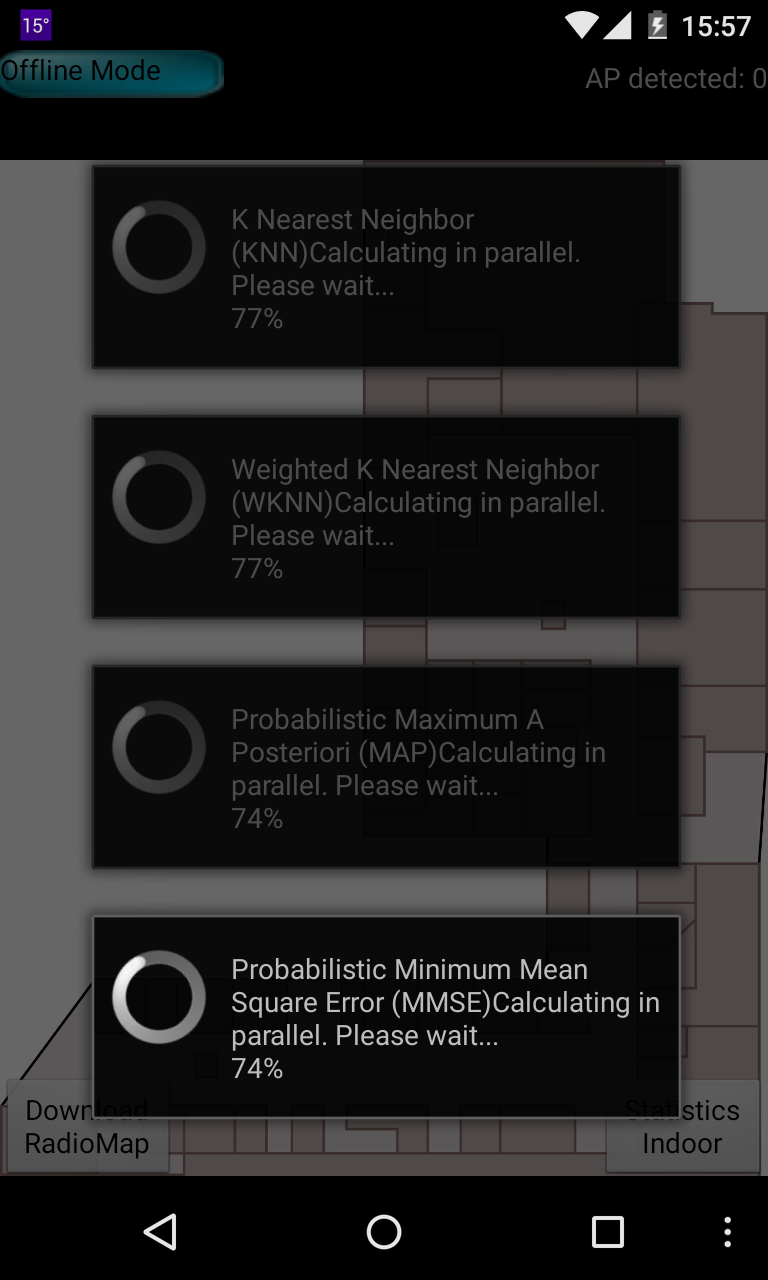
\includegraphics[width=5cm]{imatges/analisi_offline_paralel.png}
\caption{Execució d'un anàlisi en paral·lel amb AirTracker.}
\label{fig:analisi_offline_paralel}
\end{center}
\end{figure}

\subsection{Anàlisi dels resultats}

La primera deducció a la que arribam amb l'anàlisi dels resultats anteriors és que mostra un clar augment de l'error entre les estmacions en un entorn buit i un amb una quantitat considerable de persones. De totes maneres, es poden observar diferències notables depenent de l'algorisme, els paràmetres i si la posició és a un passadís o dins una tenda.

A continuació es comenten els resultats obtinguts classificats per algorisme.

\subsection{\textit{K Nearest Neighbors}}

Com es poden observar als valors de les proves realitzades (taula \ref{fig:analisi_offline_paralel}), els millors resultats amb l'algorisme \textit{K Nearest Neighbors} als passadissos s'aconsegueixen amb un valor de K=3 a un entorn sense persones (amb un error de 8,68 m.) i K=10 i K=11 en un entorn amb persones (amb un error de 9,82). En quant  l'increment de l'error entre ambdós contextos, cal destacar que excepte per valors elevats de K, on l'error de localització en un entorn buit s'incrementa constantment, l'error sempre es veu incrementat. De fet, malgrat que a partir de K=8 les mesures en un entorn amb clients arriben a ser més precises, mai arriben a l'exactitud de les millors mesures del primer context.

\begin{table}[h]
   \begin{center}
      \begin{tabular}{|l|c|c|c|}
        \hline
        \cellcolor[gray]{0.9} K & \cellcolor[gray]{0.9} Buit (m) & \cellcolor[gray]{0.9} Ple (m) & \cellcolor[gray]{0.9} Increment \\ \hline
        2  & 9,72  & 16,68 & 71,58\%  \\
        3  & 8,68  & 14,03 & 61,64\%  \\
        4  & 8,76  & 12,35 & 41,03\%  \\
        5  & 8,76  & 11,22 & 28,10\%  \\
        6  & 9,10  & 10,49 & 15,24\%  \\
        7  & 9,43  & 10,03 & 6,36\%   \\
        8  & 9,86  & 9,86  & 0,01\%   \\
        9  & 10,28 & 9,86  & -4,11\%  \\
        10 & 10,56 & 9,82  & -7,05\%  \\
        11 & 10,89 & 9,82  & -9,82\%  \\
        12 & 11,15 & 9,94  & -10,88\% \\
        13 & 11,51 & 10,17 & -11,70\% \\
        14 & 11,91 & 10,38 & -12,88\% \\
        15 & 12,28 & 10,65 & -13,28\% \\ \hline

      \end{tabular}
      
      \hspace{2pt}
      
      \begin{tabular}{|l|c|c|c|}
        \hline
        \cellcolor[gray]{0.9} K & \cellcolor[gray]{0.9} Buit (m) & \cellcolor[gray]{0.9} Ple (m) & \cellcolor[gray]{0.9} Increment \\ \hline

        2  & 13,40 & 14,95 & 11,59\\% \\
        3  & 14,38 & 15,84 & 10,12\\% \\
        4  & 15,73 & 17,29 & 9,89\\% \\
        5  & 16,66 & 18,62 & 11,80\\% \\
        6  & 18,08 & 20,06 & 10,98\\% \\
        7  & 19,19 & 20,87 & 8,73\\% \\
        8  & 20,73 & 22,19 & 7,03\\% \\
        9  & 21,89 & 23,82 & 8,82\\% \\
        10 & 23,21 & 24,92 & 7,37\\% \\
        11 & 24,40 & 26,01 & 6,61\\% \\
        12 & 25,20 & 26,56 & 5,39\\% \\
        13 & 25,83 & 27,35 & 5,87\\% \\
        14 & 26,57 & 28,02 & 5,46\\% \\
        15 & 27,14 & 28,29 & 4,24\\% \\ \hline

      \end{tabular}
      
   \end{center}
\caption{Valors de error per l'algorisme \textit{K Nearest Neighbors} en passadissos (dalt) i tendes (abaix).}
\label{tab:error_KNN}
  \end{table}

En canvi, en l'entorn dins tendes, i com s'observa clarament en els gràfics representatius de les dades (figura \ref{fig:grafic_KNN}), la tendència de l'error és similar en el dos contexts. De fet, malgrat que l'increment de l'error és proporcional a l'increment de K, l'error en les mesures del context amb clients sempre és major. 

\begin{figure}[ht]
\begin{center}
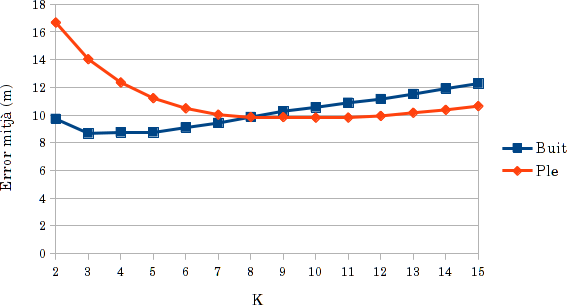
\includegraphics[width=7cm]{imatges/knn_passadis.png}
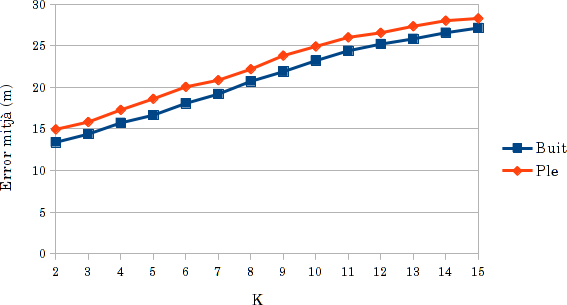
\includegraphics[width=7cm]{imatges/knn_tenda.png}
\caption{Comparació gràfica de l'error per l'algorisme \textit{K Nearest Neighbors} en passadissos (dalt) i tendes (abaix).}
\label{fig:grafic_KNN}
\end{center}
\end{figure}

La presencia de parets i altres obstacles també es fa patent al comparar els valors d'error de les mesures en passadissos i en tendes. Podem observar que, en la gran majoria de casos, les pitjors aproximacions en passadissos son, fins i tot, millors que les més acurades dins tendes.

Les imprecisions entre un entorn amb gent i sense gent també s'observen en els valors de la desviació mitjana. En tots els casos, tant en tendes com en passadissos, aquesta variable és major en els entorns amb més presència de clients, pel que podem afirmar que el nombre de persones no només afecta a la precisió mitjana de les localitzacions, sinó també a la dispersió de les estimacions.

\subsection{\textit{Weighted K Nearest Neighbors}}

En el cas de les proves amb l'algorisme \textit{Weighted K Nearest Neighbors}, la tendència és molt similar. Els gràfics (figura \ref{fig:grafic_WKNN}) mostren clarament com es segueix la mateixa tendència que amb l'anterior algorisme (\ref{fig:grafic_KNN}).

\begin{table}[h]
   \begin{center}
      \begin{tabular}{|l|c|c|c|}
        \hline
        \cellcolor[gray]{0.9} K & \cellcolor[gray]{0.9} Buit (m) & \cellcolor[gray]{0.9} Ple (m) & \cellcolor[gray]{0.9} Increment \\ \hline

        2  & 9,70  & 16,65 & 71,57\%  \\
        3  & 8,61  & 14,01 & 62,71\%  \\
        4  & 8,62  & 12,44 & 44,38\%  \\
        5  & 8,62  & 11,29 & 30,90\%  \\
        6  & 8,91  & 10,54 & 18,26\%  \\
        7  & 9,19  & 10,03 & 9,14\%   \\
        8  & 9,57  & 9,79  & 2,32\%   \\     
        9  & 9,93  & 9,73  & -1,75\%  \\
        10 & 10,20 & 9,70  & -4,90\%  \\
        11 & 10,48 & 9,68  & -7,68\%  \\
        12 & 10,73 & 9,78  & -8,82\%  \\
        13 & 11,06 & 10,00 & -9,58\%  \\
        14 & 11,42 & 10,19 & -10,78\% \\
        15 & 11,75 & 10,44 & -11,18\% \\  \hline


      \end{tabular}
      
      \hspace{10pt}
      
      \begin{tabular}{|l|c|c|c|}
        \hline
        \cellcolor[gray]{0.9} K & \cellcolor[gray]{0.9} Buit (m) & \cellcolor[gray]{0.9} Ple (m) & \cellcolor[gray]{0.9} Increment \\ \hline

        2  & 12,67 & 14,31 & 12,99\% \\
        3  & 13,39 & 14,93 & 11,54\% \\
        4  & 14,59 & 16,22 & 11,21\% \\
        5  & 15,39 & 17,33 & 12,61\% \\
        6  & 16,56 & 18,48 & 11,59\% \\
        7  & 17,50 & 19,12 & 9,26\% \\
        8  & 18,70 & 20,10 & 7,45\% \\
        9  & 19,66 & 21,43 & 9,01\% \\
        10 & 20,75 & 22,33 & 7,58\% \\
        11 & 21,76 & 23,26 & 6,88\% \\
        12 & 22,52 & 23,82 & 5,76\% \\
        13 & 23,10 & 24,49 & 6,00\% \\
        14 & 23,76 & 25,08 & 5,56\% \\
        15 & 24,28 & 25,37 & 4,49\% \\  \hline

      \end{tabular}
 \end{center}
      
\caption{Valors de error per l'algorisme \textit{Weighted K Nearest Neighbors} en passadissos (dalt) i tendes (abaix).}
\label{tab:error_WKNN}
\end{table}

Tot i així, observant els valors, podem apreciar com amb l'algorisme \textit{Weighted K Nearest Neighbors} s'aconsegueix una major precisió en tots els casos respecte a l'anterior. En passadissos, amb K=3 s'aconsegueix un error de 8,61 m. per un context sense altra presència i en un context amb clients, amb K=11, un error de 9,68 m. En el cas de tendes, els menors error mitjans s'aconsegueixen amb K=2 en ambdós contextos (12,67 m. i 14,31 m. respectivament).

\begin{figure}[ht]
\begin{center}
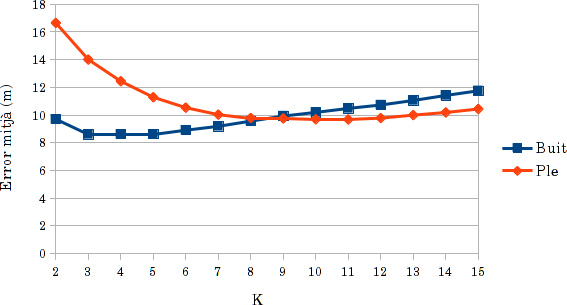
\includegraphics[width=7cm]{imatges/wknn_passadis.png}
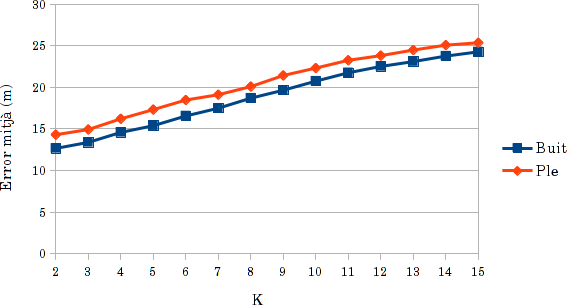
\includegraphics[width=7cm]{imatges/wknn_tenda.png}
\caption{Comparació gràfica de l'error per l'algorisme \textit{Weighted K Nearest Neighbors} en passadissos (dalt) i tendes (abaix).}
\label{fig:grafic_WKNN}
\end{center}
\end{figure}

En el cas de la dispersió de les estimacions, amb aquest algorisme observam el mateix comportament. El valor de la desviació mitjana és sempre major amb presencia de altres usuaris (arribant fins a un increment del 35,75\% en passadissos). Aquesta tendència és major als passadissos que a les tendes. Tant en l'anterior algorisme com en aquest, aquesta major dispersió de les estimacions en els passadissos es degui a la major presencia de punts de control propers que en tendes.

\subsection{\textit{Probabilistic Maximum A Posteriori}}

Realitzant el càlcul amb l'algorisme \textit{Probabilistic Maximum A Posteriori} s'obté un comportament completament diferent als anteriors. Com es pot observar, els valors de l'error mitjà minven conforme augmenta K en tots els casos (taula \ref{tab:error_MAP}), tant en passadissos com dins tendes i amb presència com amb absència d'altres usuaris.

\begin{table}[h]
  \begin{center}
      \begin{tabular}{|l|c|c|c|}
        \hline
        \cellcolor[gray]{0.9} K & \cellcolor[gray]{0.9} Buit (m) & \cellcolor[gray]{0.9} Ple (m) & \cellcolor[gray]{0.9} Increment \\ \hline
        
        2  & 51,24 & 51,22 & -0,04\%  \\
        3  & 50,47 & 51,22 & 1,49\%   \\
        4  & 37,79 & 50,14 & 32,70\%  \\
        5  & 19,88 & 41,64 & 109,43\% \\
        6  & 13,71 & 27,61 & 101,42\% \\
        7  & 12,05 & 22,63 & 87,76\%  \\
        8  & 11,92 & 21,09 & 76,87\%  \\
        9  & 11,92 & 20,68 & 73,49\%  \\
        10 & 11,92 & 20,48 & 71,78\%  \\
        11 & 11,92 & 20,48 & 71,78\%  \\
        12 & 11,92 & 20,48 & 71,78\%  \\
        13 & 11,92 & 20,48 & 71,78\%  \\
        14 & 11,92 & 20,48 & 71,78\%  \\
        15 & 11,92 & 20,48 & 71,78\%  \\ \hline

      \end{tabular}
      
      \hspace{10pt}
      
      \begin{tabular}{|l|c|c|c|}
        \hline
        \cellcolor[gray]{0.9} K & \cellcolor[gray]{0.9} Buit (m) & \cellcolor[gray]{0.9} Ple (m) & \cellcolor[gray]{0.9} Increment \\ \hline
        
        2  & 43,08 & 42,34 & -1,71\% \\
        3  & 32,43 & 32,37 & -0,19\% \\
        4  & 20,25 & 20,54 & 1,43\%  \\
        5  & 12,60 & 14,00 & 11,12\% \\
        6  & 11,38 & 12,86 & 13,06\% \\
        7  & 11,35 & 12,77 & 12,45\% \\
        8  & 11,35 & 12,77 & 12,45\% \\
        9  & 11,35 & 12,77 & 12,45\% \\
        10 & 11,35 & 12,77 & 12,45\% \\
        11 & 11,35 & 12,77 & 12,45\% \\
        12 & 11,35 & 12,77 & 12,45\% \\
        13 & 11,35 & 12,77 & 12,45\% \\
        14 & 11,35 & 12,77 & 12,45\% \\
        15 & 11,35 & 12,77 & 12,45\% \\  \hline

      \end{tabular}
      
   \end{center}
\caption{Valors de error per l'algorisme \textit{Probabilistic Maximum A Posteriori} en passadissos (dalt) i tendes (abaix).}
\label{tab:error_MAP}
\end{table}

Més particularment, els valors d'error són alts per valors petits de K, sobretot per K=2, K=3 i K=4, on les imprecisions es troben entre els 20 i els 52 metres. De totes maneres, la precisió no millora constantment, sinó que a partir de certs valors de K (K=8 a passadissos i K=7 en tendes) el valor d'error esdevé constant. A més, excepte als casos amb un error de localització major, l'error en entorns sense presència sempre esdevé menor que en cas contrari. En els casos de menor error, la presència de persones augmenta un 71,78\% la imprecisió en passadissos i un 12,45\% en tendes.

\begin{figure}[ht]
\begin{center}
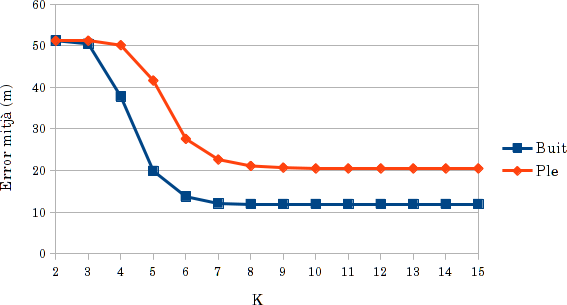
\includegraphics[width=7cm]{imatges/map_passadis.png}
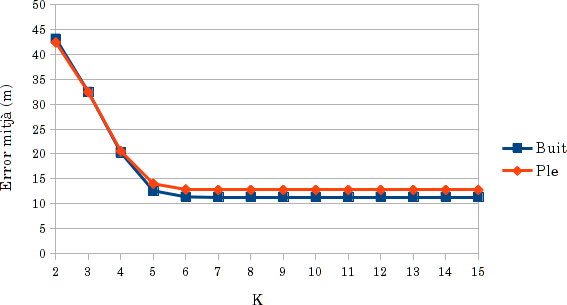
\includegraphics[width=7cm]{imatges/map_tenda.png}
\caption{Comparació gràfica de l'error per l'algorisme \textit{Probabilistic Maximum A Posteriori} en passadissos (dalt) i tendes (abaix).}
\label{fig:grafic_MAP}
\end{center}
\end{figure}

En quant a la desviació mitjana de les estimacions, en aquest cas, a l'igual que als resultats dels dos algorismes anteriors, la presència d'altres usuaris hi afecta negativament. En el cas dels millors resultats de precisió, l'augment de la dispersió augmenta un 27,61\% en passadissos i un 22,52\% dins tendes.

Malgrat que amb aquest algorisme els millors resultats de precisió són pitjors que alguns dels millors registres amb els dos anteriors algorismes, el fet de que l'error convergeixi a partir de certs valors de K pot resultar un avantatge, ja que podrem estar segurs que segurament estem obtenint els millors resultats de precisió.

\subsection{\textit{Probabilistic Minimum Mean Square Error}}


En aquest darrer cas, l'anàlisi mostra un comportament similar a l'anterior però amb particularitats. A l'igual que amb l'algorisme \textit{Probabilistic Maximum A Posteriori}, a partir de cert valor de K (K=6 en passadissos i K=5 dins tendes), l'error s'estabilitza, encara que en aquest cas segueix minvant, en menor mesura. La principal diferència s'observa en el comportament amb valors petits de K. A priori, podria semblar que valors petits de K milloren el posicionament (en un entorn sense altres usuaris s'aconsegueix un error mitjà de només 8,05 m. en passadissos), però la realitat és que si s'observen els fitxers de dades generats per AirPlace Tracker, es podrà comprovar que l'algoritme ha estat incapaç de localitzar la gran majoria de punts. De fet, com s'observa a la taula \ref{tab:error_MMSE}, en el cas de estimacions en passadissos, l'algorisme no arriba a estimar cap localització si K=2. En aquest cas, només a partir de K=6 es poden estimar totes les localitzacions.


\begin{table}[h]
  \begin{center}
      \begin{tabular}{|l|c|c|c|}
        \hline
        \cellcolor[gray]{0.9} K & \cellcolor[gray]{0.9} Buit (m) & \cellcolor[gray]{0.9} Ple (m) & \cellcolor[gray]{0.9} Increment \\ \hline
        
        3  & 8,05  & 36,40 & 352,12\% \\
        4  & 10,79 & 24,97 & 131,33\% \\
        5  & 11,82 & 21,31 & 80,28\%  \\
        6  & 11,75 & 20,19 & 71,86\%  \\
        7  & 11,77 & 20,14 & 71,15\%  \\
        8  & 11,74 & 20,25 & 72,48\%  \\
        9  & 11,69 & 20,32 & 73,78\%  \\
        10 & 11,64 & 20,34 & 74,75\%  \\
        11 & 11,58 & 20,32 & 75,37\%  \\
        12 & 11,52 & 20,28 & 76,03\%  \\
        13 & 11,46 & 20,25 & 76,71\%  \\
        14 & 11,39 & 20,21 & 77,43\%  \\
        15 & 11,32 & 20,17 & 78,20\%  \\ \hline

      \end{tabular}
      
      \hspace{10pt}
      
      \begin{tabular}{|l|c|c|c|}
        \hline
        \cellcolor[gray]{0.9} K & \cellcolor[gray]{0.9} Buit (m) & \cellcolor[gray]{0.9} Ple (m) & \cellcolor[gray]{0.9} Increment \\ \hline
        
        2  & 12,94 & 13,50 & 4,39\%  \\
        3  & 9,59  & 14,79 & 54,20\% \\
        4  & 11,52 & 15,26 & 32,46\% \\
        5  & 11,32 & 12,94 & 14,29\% \\
        6  & 11,32 & 12,69 & 12,18\% \\
        7  & 11,30 & 12,63 & 11,72\% \\
        8  & 11,29 & 12,60 & 11,59\% \\
        9  & 11,27 & 12,56 & 11,47\% \\
        10 & 11,25 & 12,53 & 11,36\% \\
        11 & 11,23 & 12,50 & 11,25\% \\
        12 & 11,21 & 12,46 & 11,14\% \\
        13 & 11,19 & 12,42 & 11,03\% \\
        14 & 11,16 & 12,37 & 10,91\% \\
        15 & 11,12 & 12,32 & 10,79\% \\ \hline

      \end{tabular}
      
   \end{center}
\caption{Valors de error per l'algorisme \textit{Probabilistic Minimum Mean Square Error} en passadissos (dalt) i tendes (abaix).}
\label{tab:error_MMSE}
\end{table}

En quant com afecta la presència d'altres usuaris a la precisió de les mesures, tant la taula \ref{tab:error_MMSE} com, més visualment, la figura \ref{fig:grafic_MMSE}, mostren que en tant en passadissos com en tendes, els resultats empitjoren amb usuaris al voltant. En els casos amb millors mesures, la diferència de precisió es troba entre un 71\% i un 78\% en passadissos i entre un 10\% i un 12\% dins tendes. Aquesta diferència en l'increment en l'error de precisió es pot deure a que l'error introduït per parets i altres obstacles estàtics dins tendes compensa l'error produït per la presència d'altres persones.

\begin{figure}[ht]
\begin{center}
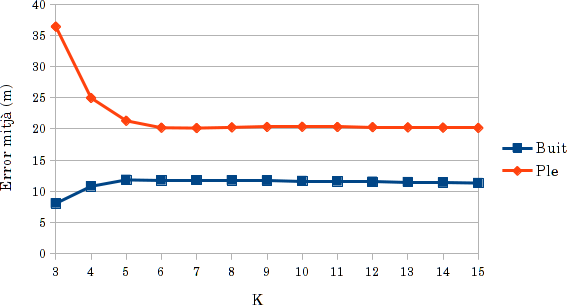
\includegraphics[width=8cm]{imatges/mmse_passadis.png}
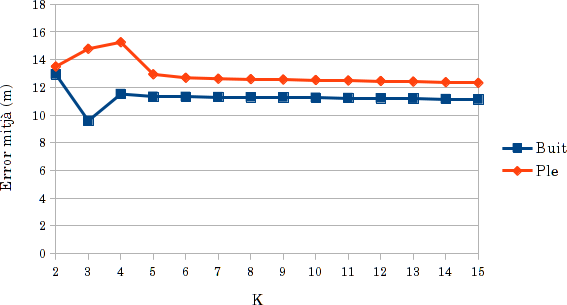
\includegraphics[width=8cm]{imatges/mmse_tenda.png}
\caption{Comparació gràfica de l'error per l'algorisme \textit{Probabilistic Minimum Mean Square Error} en passadissos (dalt) i tendes (abaix).}
\label{fig:grafic_MMSE}
\end{center}
\end{figure}

En quant a la dispersió de les estimacions, la presència de persones augmenta la desviació mitjana en tots els casos. En els millors resultats dins passadissos, l'increment de la dispersió es troba entre el 23\% i el 38\%, i en el cas de tendes l'augment de la dispersió és d'entre el 20\% i el 22\%.
